\chapter{Speichertechnologien}

Nach den Ladesystemen werden in diesem Kapitel nun die Energiespeicher für Stadtbusse betrachtet. Wie im vorigen Kapitel werden zunächst die Bewertungskriterien und die betrachteten Technologien erläutert. In Abschnitt \ref{vergleichstabellen_speichertechnologien} ab Seite \pageref{vergleichstabellen_speichertechnologien} werden die Werte aufgelistet.

Im Gegensatz zu den Ladesystemen ist die Produktvielfalt der Speichertechnologien nahezu unbegrenzt. Von daher werden hier keine konkreten Produkte verglichen, sondern es wurde versucht, die jeweils für den aktuellen Stand der Speichertechnologie relevanten Kenndaten zu finden.

\section{Bewertungskriterien} %TODO: Wie wurden die ausgewählt?
\begin{itemize}
	\item Spezifische Größen
	\begin{description}
		\item \textbf{Energiedichte}
		Für eine Batterie, die diese Technologie verwendet, d. h. inklusive Zellwände, Anschlüsse usw. Einheit: \(\frac{Wh}{l}\)
		\item \textbf{Spezifische Energie}
		Einheit: \(\frac{Wh}{kg}\)
		\item \textbf{Leistungsdichte}
		Einheit: \(\frac{W}{kg}\) %TODO: kw?
		\item \textbf{Spezifische Leistung}
		Einheit: \(\frac{W}{l}\)
	\end{description}
	\item Elektrische Parameter
	\begin{description}
		\item \textbf{Zellenspannung}
		Spannung einer Zelle dieser Technologie bei 100\% Ladezustand.
		\item \textbf{Ladung}
		Der Bereich von Ladungen (Einheit: mAh), die mit dieser Technologie gefertigt werden können. %TODO: Relevanz?
		\item \textbf{Nennladestrom}
		Ladestrom, mit dem im Bereich zwischen 20\% und 80\% der verfügbaren Kapazität geladen wird. Angabe in Teil an der Ladung\\
		Beispiel: Wenn eine Batterie mit 1400mAh Ladung werden mit 140mA aufgeladen wird, entspricht dies einem Ladestrom von 0,1C.
		\item \textbf{Besondere Ladeströme}
		Ladeströme unter anderen Bedingungen, zum Beispiel bei geringem oder hohem Ladezustand oder besonderer Temperatur.
		\item \textbf{Balancing}
		Wenn eine Batterie aus mehreren Zellen aufgebaut ist, müssen die Ladezustände zwischen den Zellen angeglichen werden. Je nach Technologie kann das durch Überladen erfolgen oder erfordert eine Verbindung von jeder Zelle zum Ladegerät.
		\item \textbf{Innenwiderstand} %TODO: Effizienz nur über Innenwiderstand?
	\end{description}
	\item Sicherheit und Zuverlässigkeit
	\begin{description}
		\item \textbf{Kapazitätsverlust, zeitlich}
		Zeitabhängiger Kapazitätsverlust bei Normalbedingungen, Angabe in Prozent pro Jahr%TODO: Bedingungen
		\item \textbf{Kapazitätsverlust, nutzungsabhängig}
		Nutzungsabhängiger Kapazitätsverlust bei maximaler Lade- und Entladestaärke und vollen Ladezyklen, Angabe in Prozent pro Ladezyklus %TODO: Bedingungen
		\item \textbf{Verhalten bei Übertemperatur}
		\item \textbf{Unfallverhalten}
		\item \textbf{Verhalten bei Zellenfehler}
		\item \textbf{Selbstentladung}
	\end{description}
\end{itemize}

\section{Betrachtete Technologien}
Im folgenden Abschnitt werden die Grundlagen und die Einsatzgeschichten der verschiedenen Speichertechnologien kurz erläutert. Die Technologien sind nach dem genutzten physikalischen Effekt aufgeteilt \cite{Sterner:2014}[S. 35f]. Im realen Betrieb werden manchmal auch Kombinationen von verschiedenen Speichertechnologien eingesetzt, um dem hohen Leistungsbedarf beim Anfahren und bei der Bremsenergierückgewinnung gerecht zu werden.

\subsection{Mechanisch – Schwungradspeicher} %TODO: Quellen, warum endete die Gyrobuserprobung
In Bussen kann mechanische Energie mit einem Schwungrad gespeichert werden\footnote{Es gibt auch Prototypen von Pressluftspeichern in kleineren Fahrzeugen, in Bussen werden sie jedoch nur als Teil eines Hybridantriebs eingesetzt und hier nicht weiter betrachtet \cite{Sebastian-Naumann:2014}[S. 14].}. Die Energieübertragung erfolgt durch eine elektrische Motor- und Generatoreinheit. Moderne Schwungräder werden aus gewickelten Karbonfasern hergestellt und in Vakuumgehäusen magnetisch gelagert, sie erreichen hohe Drehzahlen und geringe Reibungsverluste \cite{993788}. Im Falle eines berstenden Schwungrades muss das Gehäuse die gesamte Energie innerhalb von Sekundenbruchteilen aufnehmen, ohne selbst zu bersten. Dies erfordert sehr schwere Gehäuse, die die spezifische Energie und Leistung eines tatsächlichen Systems stark reduzieren. Der Schwungradspeicher wurde in den fünfziger Jahren im Gyrobus im schweizerischen Yverdon auf einer acht Kilometer langen Linie erprobt. Die Strecke wurde erfolgreich zurückgelegt, die damalige Technologie war jedoch sehr wartungsaufwändig und weniger effizient als ein Oberleitungsbus. Aktuell wird der Schwungradspeicher nur als Teil eines hybriden Antriebsstrangs eingesetzt \cite{tub_aleph001746639}[S. 216].

\subsection{Elektrisch – Kondensator} %TODO: Quellen
Der Kondensator ist ein rein elektrischer Energiespeicher. Im klassischen Plattenkondensator werden zwei durch einen festes Dielektrikum getrennte Platten elektrisch aufgeladen, die Ladung kann später in Strom umgewandelt werden. Kondensatoren haben eine hohe spezifische Leistung, aber eine sehr geringe spezifische Energie. In Bussen werden sogenannte Superkondensatoren verwendet, die statt eines festen Dielektrikums ein Elektrolyt (meist eine Salz-Wasser-Lösung) verwenden. Die im Elektrolyt gelösten Ionen werden von der geladenen Platte angezogen, können sie jedoch aufgrund der umgebenden Wasserschicht nicht erreichen (siehe Abbildung \ref{abb_doppelschicht}). Da der Abstand zwischen Platte un Ionen extrem klein ist, entsteht eine sehr hohe elektrische Kapazität. Eine weitere Kapazitätssteigerung wird durch die Einlagerung von einigen Elektronen des Elektrolyts in den Leiterplatten erreicht \cite{Sterner:2014}[S. 167f].

\begin{figure}\centering
	 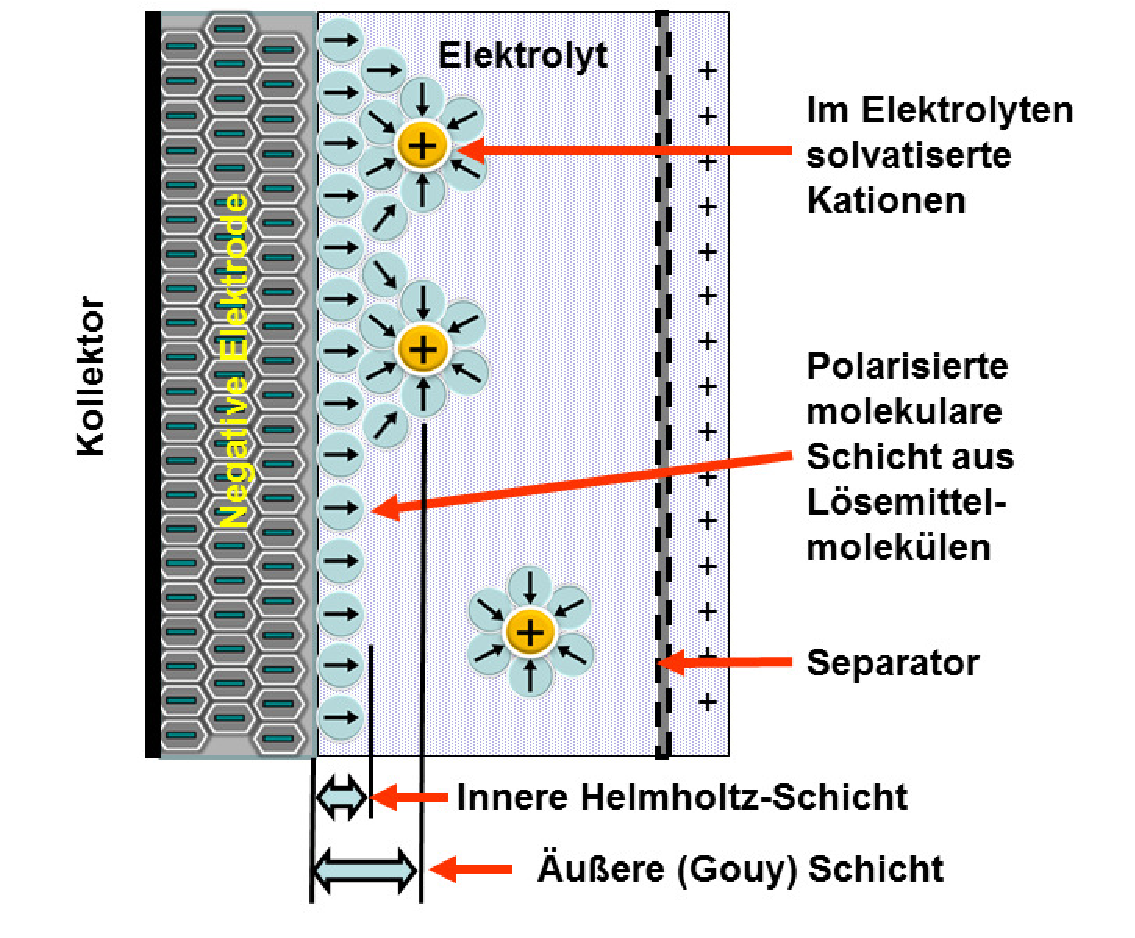
\includegraphics[width=0.5\textwidth]{Doppelschicht-Prinzipdarstellung}
	 \caption{Prinzipdarstellung der Doppelschichtkapazität. Quelle: Elcap (Own work) CC BY-SA 3.0, via Wikimedia Commons}
	 \label{abb_doppelschicht}
\end{figure}

In Shanghai werden Busse mit dieser Technologie seit 2008 im Linienverkehr eingesetzt, daneben werden Superkondensatoren für kurzzeitige Einsätze mit hohem Leistungsbedarf, zum Beispiel zur Bremsenergierückgewinnung oder zur Überbrückung stromloser Stellen in Trolleybussen eingesetzt \cite{Barminer-Busgesellschaft:2012}.

\subsection{Elektrochemisch – Batterie} %TODO: Besser
Batterien bestehen aus zwei Elektroden aus meist verschiedenen Metallen. Zwischen den Elektroden befindet sich ein Elektrolyt, in dem sich Ionen von der einen Elektrode zur anderen bewegen können. Durch die Bewegung der Ionen wird Ladung übertragen und an den Klemmen der Batterie entsteht eine Spannung. Hier werden nur wiederaufladbare Batterien (sogenannte Sekundärbatterien) betrachtet\footnote{Die Begriffe Batterie, Akkumulator und Akku werden austauschbar verwendet.}, die für den Einsatz in Fahrzeugen geeignet sind. In der Herstellung werden einzelne Batteriezellen in parallel- und Reihenschaltung zu Batteriemodulen zusammengefasst, um höhere Ströme und Spannungen zu erreichen. Die Bauformen sind sehr unterschiedlich, meist werden jedoch gewickelte oder ineinander geschachtelte Flache Elektroden verwendet um die Oberflächen und damit die Stromstärke zu maximieren \cite{Sterner:2014}[S. 209ff].

\subsubsection{Blei-Säure}
Der Blei-Säure-Akkumulator besteht aus zwei Bleielektroden in einer Schwefelsäurelösung. Vor dem ersten Aufladen bildet sich an beiden Elektronen Bleisulfat ($PbSO_4$). Die Elektrodengleichungen sind in Tabelle \ref{Pb} aufgeführt \cite{KiehneBattery}[S. 50].

\begin{table}\centering
  \begin{tabularx}{\linewidth}{XrcX}
  	                   &                       $geladen$ & $\rightleftarrows$ & $entladen$             \\
  	Negative Elektrode & $PbO_2 + H_2SO_4 + 2H^+ + 2e^-$ & $\rightleftarrows$ & $PbSO_4 + 2H_2O$       \\
  	Positive Elektrode &                  $Pb + H_2SO_4$ & $\rightleftarrows$ & $PbSO_4 + 2H^+ + 2e^-$ \\ \midrule
  	Zellenreaktion     &         $Pb + PbO_2 + 2H_2SO_4$ & $\rightleftarrows$ & $2PbSO_4 + 2H_2O$      \\
  \end{tabularx}
  \caption{Elektrodengleichungen der Blei-Säure-Batterie}
  \label{Pb}
\end{table}

Im Gegensatz zu den meisten anderen Batterien transportiert hier der Elektrolyt nicht nur die Ionen, sondern ist selbst an der Reaktion beteiligt.

Im geladenen Zustand wird das enthaltene Wasser elektrolytisch zu Wasserstoff und Sauerstoff zerlegt. Dieser Wasserverlust muss durch periodisches Nachfüllen oder Rekombination der Gase zu Wasser ausgeglichen werden. Vorteil der Gasentwicklung ist, das so durch Überladen die Spannungen verschiedener Zellen angeglichen werden können, da die Energie des Überladevorgangs in die Wasserspaltung geführt wird \cite{tub_aleph001746639}[S. 182].

Der Blei-Säure-Akkumulator ist eine der ältesten wiederaufladbaren Batterietechnologien und wurde in allen frühen Elektrobussen eingesetzt, zum Beispiel im weltweit ersten Batteriebus, der ab 1900 auf der Strecke Anhalter Bahnhof – Stettiner Bahnhof (heute: Nordbahnhof) in Berlin erprobt wurde \cite{Risch:1957}[S. 8f].

\subsubsection{Nickel-Cadmium}
Die Elektroden bestehen aus Nickelhydroxid und Cadmiumhydroxid in einem alkalischen, wässrigen Elektrolyt, dass nicht an der Reaktion beteiligt ist, sondern nur dem Ionentransport dient. Die Reaktionsgleichungen sind in Tabelle \ref{NiCd} aufgeführt \cite{Sterner:2014}[S.233].

\begin{table}\centering
  \begin{tabularx}{\linewidth}{XrcX}
  	                   &               $geladen$ & $\rightleftarrows$ & $entladen$             \\
  	Negative Elektrode &            $Cd + 2OH^-$ & $\rightleftarrows$ & $Cd(OH)_2 + 2e^-$      \\
  	Positive Elektrode & $2NiOOH + 2H_2O + 2e^-$ & $\rightleftarrows$ & $2Ni(OH)_2 + 2OH^-$    \\ \midrule
  	Zellenreaktion     &   $Cd + 2NiOOH + 2H_2O$ & $\rightleftarrows$ & $Cd(OH)_2 + 2Ni(OH)_2$ \\
  \end{tabularx}
  \caption{Elektrodengleichungen der Nickel-Cadmium-Batterie}
  \label{NiCd}
\end{table}

Wie bei Blei-Säure-Batterien wird der Elektrolyt in Wasserstoff und Sauerstoff zerlegt, es sind offenen Bauformen und geschlossene Bauformen mit interner Rekombination vorhanden.

Die Nickel-Cadmium Batterie weist eine weit höhere spezifische Energie als die Blei-Säure-Batterie auf, wird jedoch in elektrischen Bussen nicht verwendet.

\subsubsection{Nickel-Metallhydrid}
Die Nickel-Mettalhydridbatterie verwendet wie die Nickel-Cadmiumbatterie eine Nickel(oxy)hydroxidelektrode und einen alkalischen Elektrolyt. Der Unterschied ist, das hier statt giftigem Cadmium(hydroxid) in der negativen Elektrode Metall eingesetzt, in dem $H^+$-Ionen zu Wasserstoff reduziert und eingelagert werden. Dieser Hydrierung genannte Vorgang tritt in vielen verschiedenen Metallen und Legierungen auf. In diesen Batterien wird meist eine Legierung aus seltenen Erden und Nickel verwendet \cite{KiehneBattery}[S. 85ff]. Die Reaktionsgleichungen sind in Tabelle \ref{NiMH} aufgeführt \cite{Sterner:2014}[S. 245].

\begin{table}\centering
  \begin{tabularx}{\linewidth}{XrcX}
  	                   &              $geladen$ & $\rightleftarrows$ & $entladen$        \\
  	Negative Elektrode &          $M(H) + OH^-$ & $\rightleftarrows$ & $M + H_2O + e^-$  \\
  	Positive Elektrode &   $NiOOH + H_2O + e^-$ & $\rightleftarrows$ & $Ni(OH)_2 + OH^-$ \\ \midrule
  	Zellenreaktion     & $M(H) + NiOOH + 2H_2O$ & $\rightleftarrows$ & $M + Ni(OH)_2$    \\
  \end{tabularx}
  \caption{Elektrodengleichungen der Nickel-Metallhydrid-Batterie}
  \label{NiMH}
\end{table}

Da die Hydrierung bei Drücken von bis zu 10 Bar stattfindet, gibt es nur geschlossene Bauformen. Der Nickel-Metallhydrid-Akku wird in mehreren Hybridfahrzeugen verwendet, zum Beispiel im Toyota Prius.

\subsubsection{Lithium-Ionen}
In Lithium-Ionen-Akkus erfolgt der Ladungstransfer durch $Li^+$-Ionen, die durch ein Elektrolyt aus Lithiumsalzen in organischen Lösungsmitteln wandern. Der Elektrolyt ist häufig in ein Polymer eingelagert, das so entstandene Gel dient sowohl als Elektrolyt als auch zur mechanischen Separation der Elektroden\footnote{Es wird auch an einphasigen, festen Polymerelektrolyten geforscht, mit deren geringer Dicke eine hohe Energiedichte erreicht werden könnte. Diese Technologie wird jedoch noch nicht kommerziell eingesetzt.} \cite{xu2004nonaqueous}. Im Gegensatz zu den anderen Batterietypen, bei denen das Elektrodenmaterial oxidiert und reduziert wird, wandert hier das Metall selber von Elektrode zu Elektrode. Reine Lithiumelektroden würden sich auflösen und dadurch ihre Form verlieren, von daher werden für positive und negative Elektrode verschiedene Materialien verwendet, in denen die Lithiumionen eingelagert werden \cite{KiehneBattery}[S. 408, 440ff].

\paragraph{Geschichtete Oxide}

\begin{figure}\centering
	 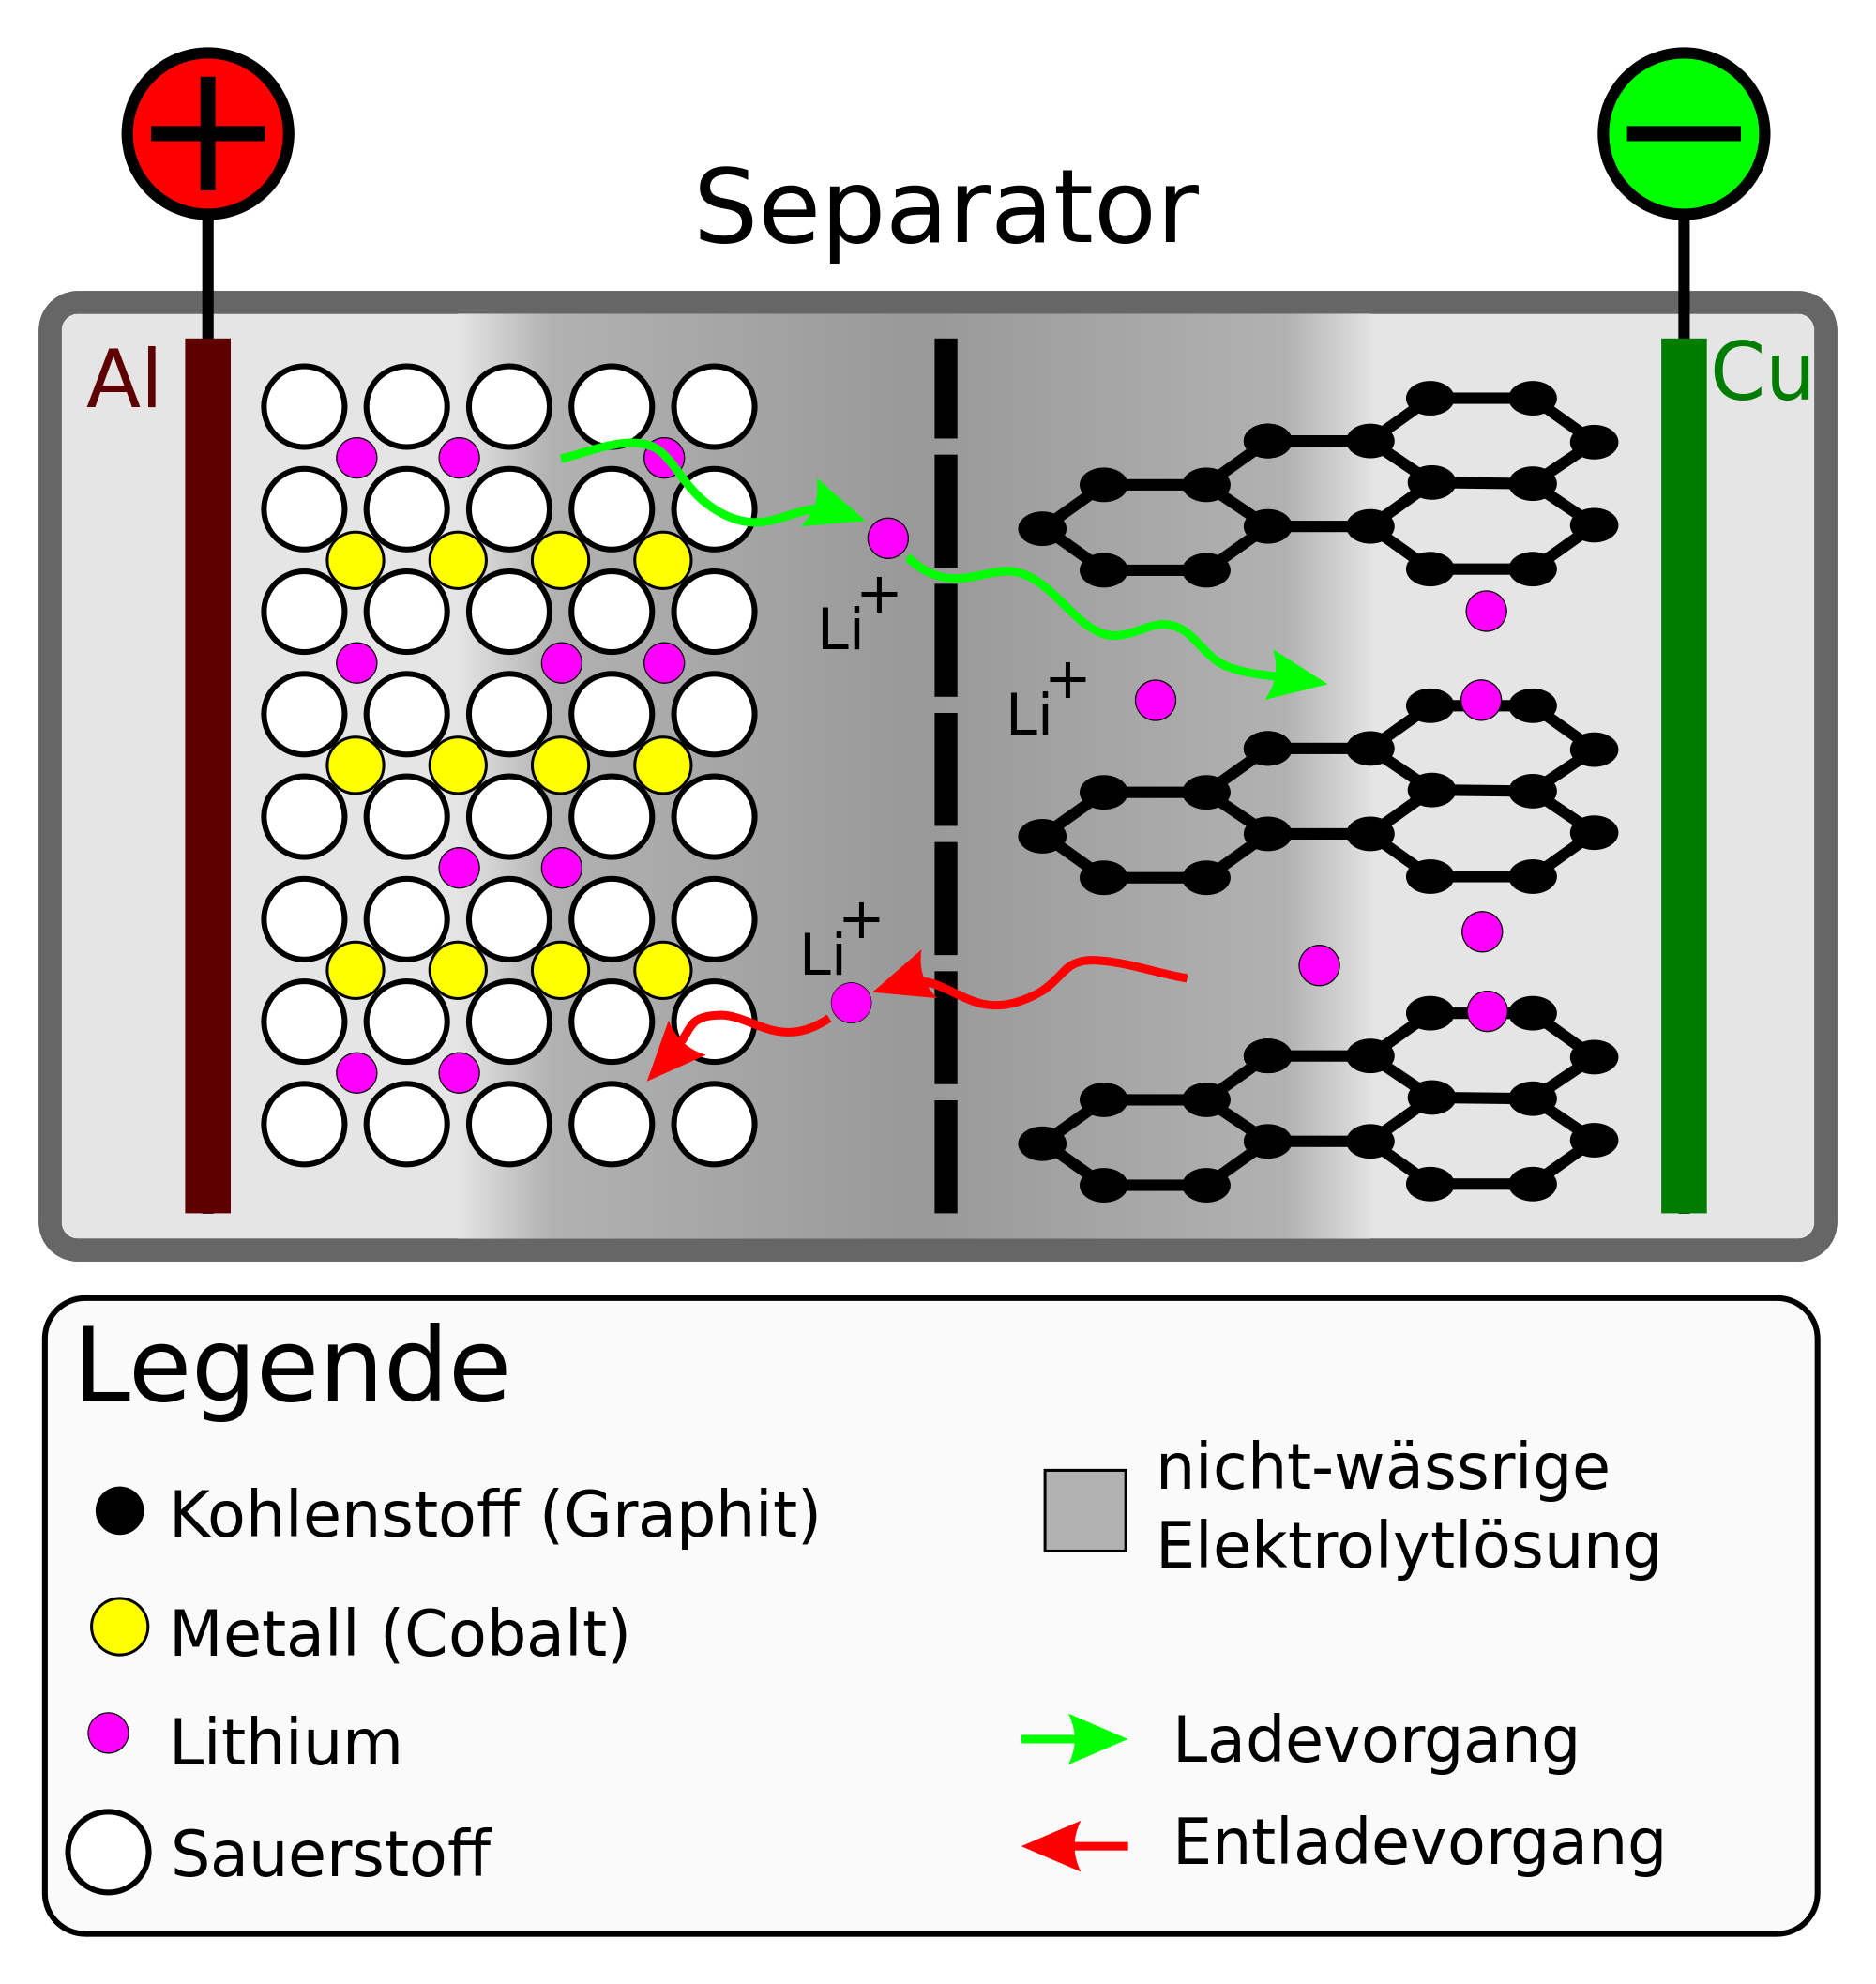
\includegraphics[width=0.5\textwidth]{LiCoO2}
	 \caption{Prinzipdarstellung eines Lithium-Inonen-Akkus mit Kobaltoxid in der positiven Elektrode. Quelle: Cepheiden (Own work) CC BY-SA 2.0, via Wikimedia Commons}
	 \label{abb_LiCoO2}
\end{figure}

In kleinen und mittelgroßen Akkus werden meist positive Elektroden aus Lithium-Metalloxiden verwendet. Diese haben eine kubische Kristallstruktur, das Lithium wird zwischen den Sauerstoffatomen eingelagert. Positive Elektroden aus $LiCoO_2$ werden seit den 90er Jahren in kommerziellen Lithiumakkus verwendet. Daneben werden auch $LiMn_2O_4$, und $LiMnO_2$ verwendet, mit denen man günstigere Akkus auf Kosten der spezifischen Energie herstellen kann \cite{whittingham2004lithium}. %TODO: Welche Busse?

Die negative Elektrode besteht in allen Fällen aus Graphit, die Lithiumionen werden zwischen den verschiedenen Schichten der Graphitkristalle eingelagert. Es werden verschiedene Größen von Graphitkristallen und auch andere Modifikationen von Kohlenstoff verwendet \cite{Sterner:2014}[S. 252]. Ein Lithium-Kobaltoxid-Akku ist in Abbildung \ref{abb_LiCoO2} schematisch dargestellt.

\paragraph{Lithium-Eisenphosphat}
Lithium-Eisenphosphat ($LiFePO_4$) ist ein neues Material für die positive Elektrode. Die theoretische spezifische Energie ist ähnlich der von geschichteten Oxiden, aktuell wird jedoch nur eine niedrigere spezifische Energie erreicht \cite{Tie201382}. In der negativen Elektrode wird Graphit verwendet. Aufgrund des niedrigen Preises von Eisen sind diese Batterien gut für elektrische Fahrzeuge geeignet und werden zum Beispiel in den elektrischen Bussen von \textsc{BYD} verwendet \cite{bydSpecs}.

\paragraph{Lithium-Titanat}
Im Gegensatz zu den vorigen Materialien ist Lithium-Titanat ($Li_4Ti_5O_{12}$) kein Material für die positive Elektrode, sondern ersetzt das Graphit in der negativen Elektrode und wird meist in Kombination mit $LiCoO_2$ eingesetzt. Diese Technologie bietet eine niedrigere spezifische Energie, dafür eine weit höhere spezifische Lade- und Entladeleistung \cite{veneri2012charging}. Damit ist sie insbesondere für Stadtbusse mit Gelegenheitsladung interessant und wird zum Beispiel von \textsc{Proterra} in elektrischen Stadtbussen eingesetzt \cite{protCat}.

\subsubsection{Natrium-Nickelchlorid}
Die Natrium-Nickelcloridbatterie (auch als ZEBRA-Batterie bekannt) ist eine Hochtemperaturbatterie. Sie verwendet als Elektrolyt feste Alumiumkeramik, die nur für $Na^+$-Ionen durchlässig ist. Die Elektroden bestehen aus flüssigem Kochsalz und Nickel, der ebenfalls in flüssigem Kochsalz gelagert ist. Die Reaktionsgleichungen sind in Tabelle \ref{ZEBRA} aufgeführt \cite{KiehneBattery}[S. 257ff].

\begin{table}\centering
  \begin{tabularx}{\linewidth}{XrcX}
  	                   &       $geladen$ & $\rightleftarrows$ & $entladen$           \\
  	Negative Elektrode & $NiCl_2 + 2e^-$ & $\rightleftarrows$ & $2Cl^- + 2Na^+ + Ni$ \\
  	Positive Elektrode &           $2Na$ & $\rightleftarrows$ & $2e^-$               \\ \midrule
  	Zellenreaktion     &  $2Na + NiCl_2$ & $\rightleftarrows$ & $Ni + 2NaCl$
  \end{tabularx}
  \caption{Elektrodengleichungen der Natrium-Nickelchlorid-Batterie}
  \label{ZEBRA}
\end{table}

Damit das Kochsalz flüssig bleibt, muss die Batterie permanent geheizt werden, es werden immer ca. 100W pro 20kWh Kapazität zum Heizen benötigt. Im Gegenzug besitzt dieser Batterietyp eine hohe Lebensdauer und Leistungsdichte. In Kalifornien wurde ein Schulbus mit dieser Batterietechnologie erprobt \cite{Electric-Transportation-Department:2004}.

\section{Vergleichstabellen}   %TODO: AUSFÜLLEN!
\label{vergleichstabellen_speichertechnologien}

Die meisten Daten stammen aus "`A review of energy sources and energy management system in electric vehicles"' \cite{Tie201382}, andere Quellen sind in der Tabelle jeweils für eine Technologie oder einen spezifischen Datenpunkt angegeben.

\begin{table}\centering
	\begin{tabularx}{\linewidth}{lXXXX}
		%TODO: ??? bei Wh/l
		\toprule
		\multirow{2}{*}{Technologie} & spez. Energie   & spez. Leistung & Energiedichte  & Leistungsdichte \\
		                             & $\frac{Wh}{kg}$ & $\frac{W}{kg}$ & $\frac{Wh}{l}$ & $\frac{W}{l}$   \\ \midrule
		\textbf{Mechanisch}          &                 &                &                &  \\
		Schwungrad                   & 10 -- 150       & 2 -- 10000     &                &  \\
		\textbf{Elektrostatisch}     &                 &                &                &  \\
		Superkondensator             & 10 -- 15        & 1000 -- 2000   &                &  \\
		\textbf{Elektrochemisch}     &                 &                &                &  \\
		Blei-Säure                   & 50              & 150            & 100            &  \\
		Nickel-Cadmium               & 50 -- 80        & 200            & 300            &  \\
		Nickel-Metallhydrid          & 70 -- 95        & 200 -- 300     & 180 -- 220     &  \\
		Li-Ion -- $LiCoO_2$          & 118 -- 250      & 200 -- 430     & 200 -- 400     &  \\
		Li-Ion -- $LiFePO_4$         & 120             & 2000 -- 4500   & 220            &  \\
		Li-Ion -- $Li_4Ti_5O_{12}$   & 80 -- 100       & 4000           &                &  \\
		Ni-NaCl (ZEBRA)              & 90 -- 120       & 155            & 160            &  \\ \bottomrule
	\end{tabularx}
	\caption{Übersicht Ladesysteme}
\end{table}